\section{Proposed \method\ Methodology}
The methodology connects four components. A constrained Markov decision
process specifies what each role observes and controls. Physical and virtual
queues determine a shared slot reward through the Lyapunov construction.
Hybrid MADDPG uses this reward to learn routing, resource, and flight
decisions, and a deterministic feasibility controller checks the resulting
proposals before execution. Domain randomization exposes this policy to the
declared operating family during training.

\subsection{Constrained Markov Decision Process and Agent Roles}
The controller is represented by
\begin{equation}
\mathcal M=\langle\mathcal S,\{\mathcal O_g\}_{g\in\mathcal G},
\mathcal A,\mathcal P,\mathcal R,\gamma\rangle,
\qquad \mathcal G=\{\mathsf V,\mathsf R,\mathsf U\},
\label{eq:cmdp}
\end{equation}
where $\mathcal S$ is the centralized state space, $\mathcal O_g$ is the
observation space of role $g$, $\mathcal A$ is the joint hybrid action space,
$\mathcal P$ is the transition kernel, $\mathcal R$ is the common reward, and
$\gamma\in[0,1)$ is the discount factor.

\subsubsection{State and Local Observations}
A sufficient simulator state at the start of slot $t$ is
\begin{align}
s_t=\big(&\{Q_j(t)\}_{j\in\mathcal J},
\{\ell_i,\sigma_i(t),b_i^{\rm rem}(t),
c_i^{\rm rem}(t)\}_i,\nonumber\\
&\{\vect p_v(t)\}_v,
\{\vect p_u(t),\vect u_u(t),B_u(t),Z_u(t),m_u(t)\}_u,\nonumber\\
&
\vect c_t,t/T\big),
\label{eq:method_state}
\end{align}
where $\sigma_i$ is task stage, $m_u$ is UAV activity mode, and $\vect c_t$
contains channel and available-resource summaries. Variable task sets are
padded to the configured maximum and accompanied by masks; padding never
removes a task from the physical queues.

Actor $h$ in role $g$ receives $o_h(t)=\mathcal O_h(s_t)$. A vehicle observes
its ingress/local workload, visible task features, position, and advertised
edge summaries. An RSU observes its staged and compute queues. A UAV also
observes its charge, virtual deficit, return reserve, motion state, nearby
agents, and service queues. Centralized critics receive the complete state and
joint action only during training.

\subsubsection{Hybrid Joint Action Space}
Let $i_v(t)$ denote the eligible head task of vehicle $v$. The role actions are
\begin{align}
a_v(t)&=\left(h_i,x_i^{L},\{x_{ir}^{R}\}_{r},
\{x_{iu}^{U}\}_{u},\rho_i\right),\nonumber\\
a_r(t)&=\{w_{ir}(t)\}_{i\in\mathcal I_r(t)},\nonumber\\
a_u(t)&=\left(\bar f_u(t),\{w_{iu}(t)\}_{i\in\mathcal I_u(t)},
\vect u_u(t)\right),\nonumber\\
\vect a_t&=\left(\{a_v\}_v,\{a_r\}_r,\{a_u\}_u\right).
\label{eq:joint_action}
\end{align}
Vehicle actions combine categorical holding/destination selection with the
continuous UAV-local fraction $\rho_i$. RSU and UAV shares lie on a simplex;
UAV frequency and velocity are bounded continuous decisions. State-dependent
masks remove absent tasks, uncovered nodes, returning UAVs, and destinations
without an admissible energy contingency.

\subsubsection{Transition and Cooperative Reward}
The repaired action $a_t^{\rm exec}=\mathcal H(s_t,\hat a_t)$ induces
\begin{align}
s_{t+1}&\sim\mathcal P(\cdot\mid s_t,a_t^{\rm exec}),
&r_t&=-G(t),\nonumber\\
J(\pi)&=\E_\pi\!\left[\sum_{t=0}^{T-1}\gamma^t r_t\right].
\label{eq:transition_reward}
\end{align}
where $G(t)$ is the drift-plus-penalty score defined below. The transition
commits radio and computation service, task-stage movement, flight, battery
expenditure, end-of-slot harvesting, and new arrivals in the causal order of
Section~III. Every role receives the same reward, computed from the action
that was actually executed.

\subsection{Lyapunov Drift-Plus-Penalty Transformation}
\subsubsection{Virtual Net-Energy Deficit}
For UAV $u$, introduce
\begin{equation}
Z_u(t+1)=\left[Z_u(t)+E_u(t)-H_u(t)-\bar e_u\right]^+,
\label{eq:virtual_energy_correct}
\end{equation}
where $E_u(t)$ is executed expenditure, $H_u(t)$ is realized end-of-slot
replenishment, and $\bar e_u$ is the permitted average net draw. Physical
charge still follows the battery-causality equations of Section~III; $Z_u$ is
an accounting queue and cannot supply energy.

Using fixed scales $Q^*>0$ and $E^*>0$, define
\begin{align}
q_j&=Q_j/Q^*, & z_u&=Z_u/E^*,\nonumber\\
y_j&=(A_j-S_j)/Q^*,
&e_u&=(E_u-H_u-\bar e_u)/E^*.
\end{align}
The quadratic Lyapunov function and conditional drift are
\begin{align}
L(t)&=\frac12\sum_jq_j^2(t)+\frac12\sum_uz_u^2(t),\nonumber\\
\Delta_L(t)&=\E[L(t+1)-L(t)\mid s_t].
\end{align}
Applying the squared positive-part inequality yields
\begin{align}
\Delta_L(t)+V\E[C(t)\mid s_t]
&\le D_0+\E[G(t)\mid s_t],\label{eq:dpp_bound_new}\\
G(t)&=VC(t)+w_Q\sum_jq_j(t)y_j(t)\nonumber\\
&\quad+w_Z\sum_uz_u(t)e_u(t),
\label{eq:dpp_score_new}
\end{align}
where $D_0$ is action independent, $C(t)$ is the normalized instantaneous
cost defined in Section~IV, and the implementation uses $w_Q=w_Z=1$ unless
an ablation states otherwise. Large physical queues increase the value of
service; a large virtual deficit increases the cost of net UAV energy. The
trade-off weight $V$ balances immediate cost and backlog pressure.

\begin{figure*}[!t]
\centering
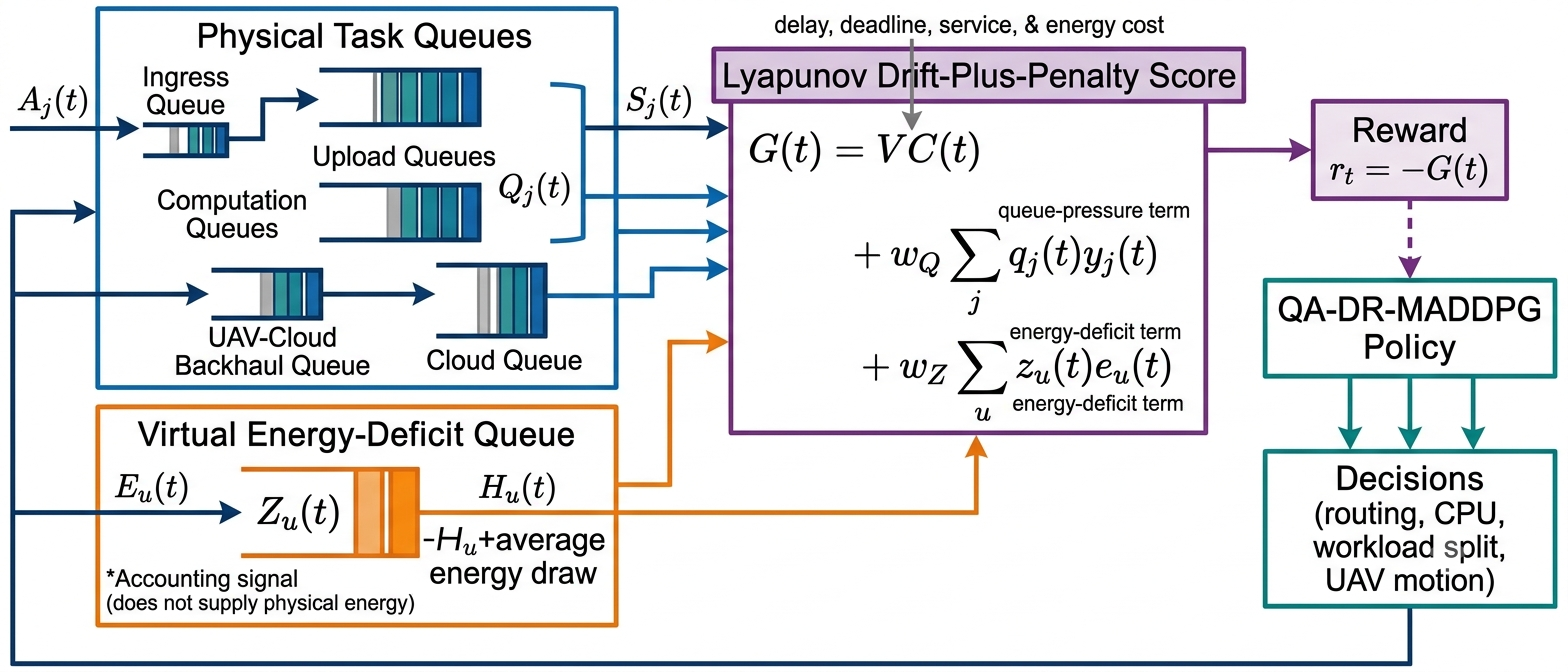
\includegraphics[width=0.94\textwidth]{Physical and virtual queue feedback diagram.png}
\caption{Queue-aware Lyapunov feedback used by the common reward. Physical
task queues and the virtual net-energy deficit enter the drift-plus-penalty
score, whose negative is supplied to the cooperative controller. Executed
decisions then determine queue service and energy expenditure in the next
transition.}
\label{fig:lyapunov_feedback}
\end{figure*}

\subsection{Hybrid MADDPG Decision Engine}
Fig.~\ref{fig:controller_architecture} shows the complete centralized-training
and decentralized-execution architecture. Role-shared actors create a joint
hybrid proposal, the deterministic feasibility layer produces the executed
action, and centralized critics learn from replay containing both versions.

\begin{figure*}[!t]
\centering
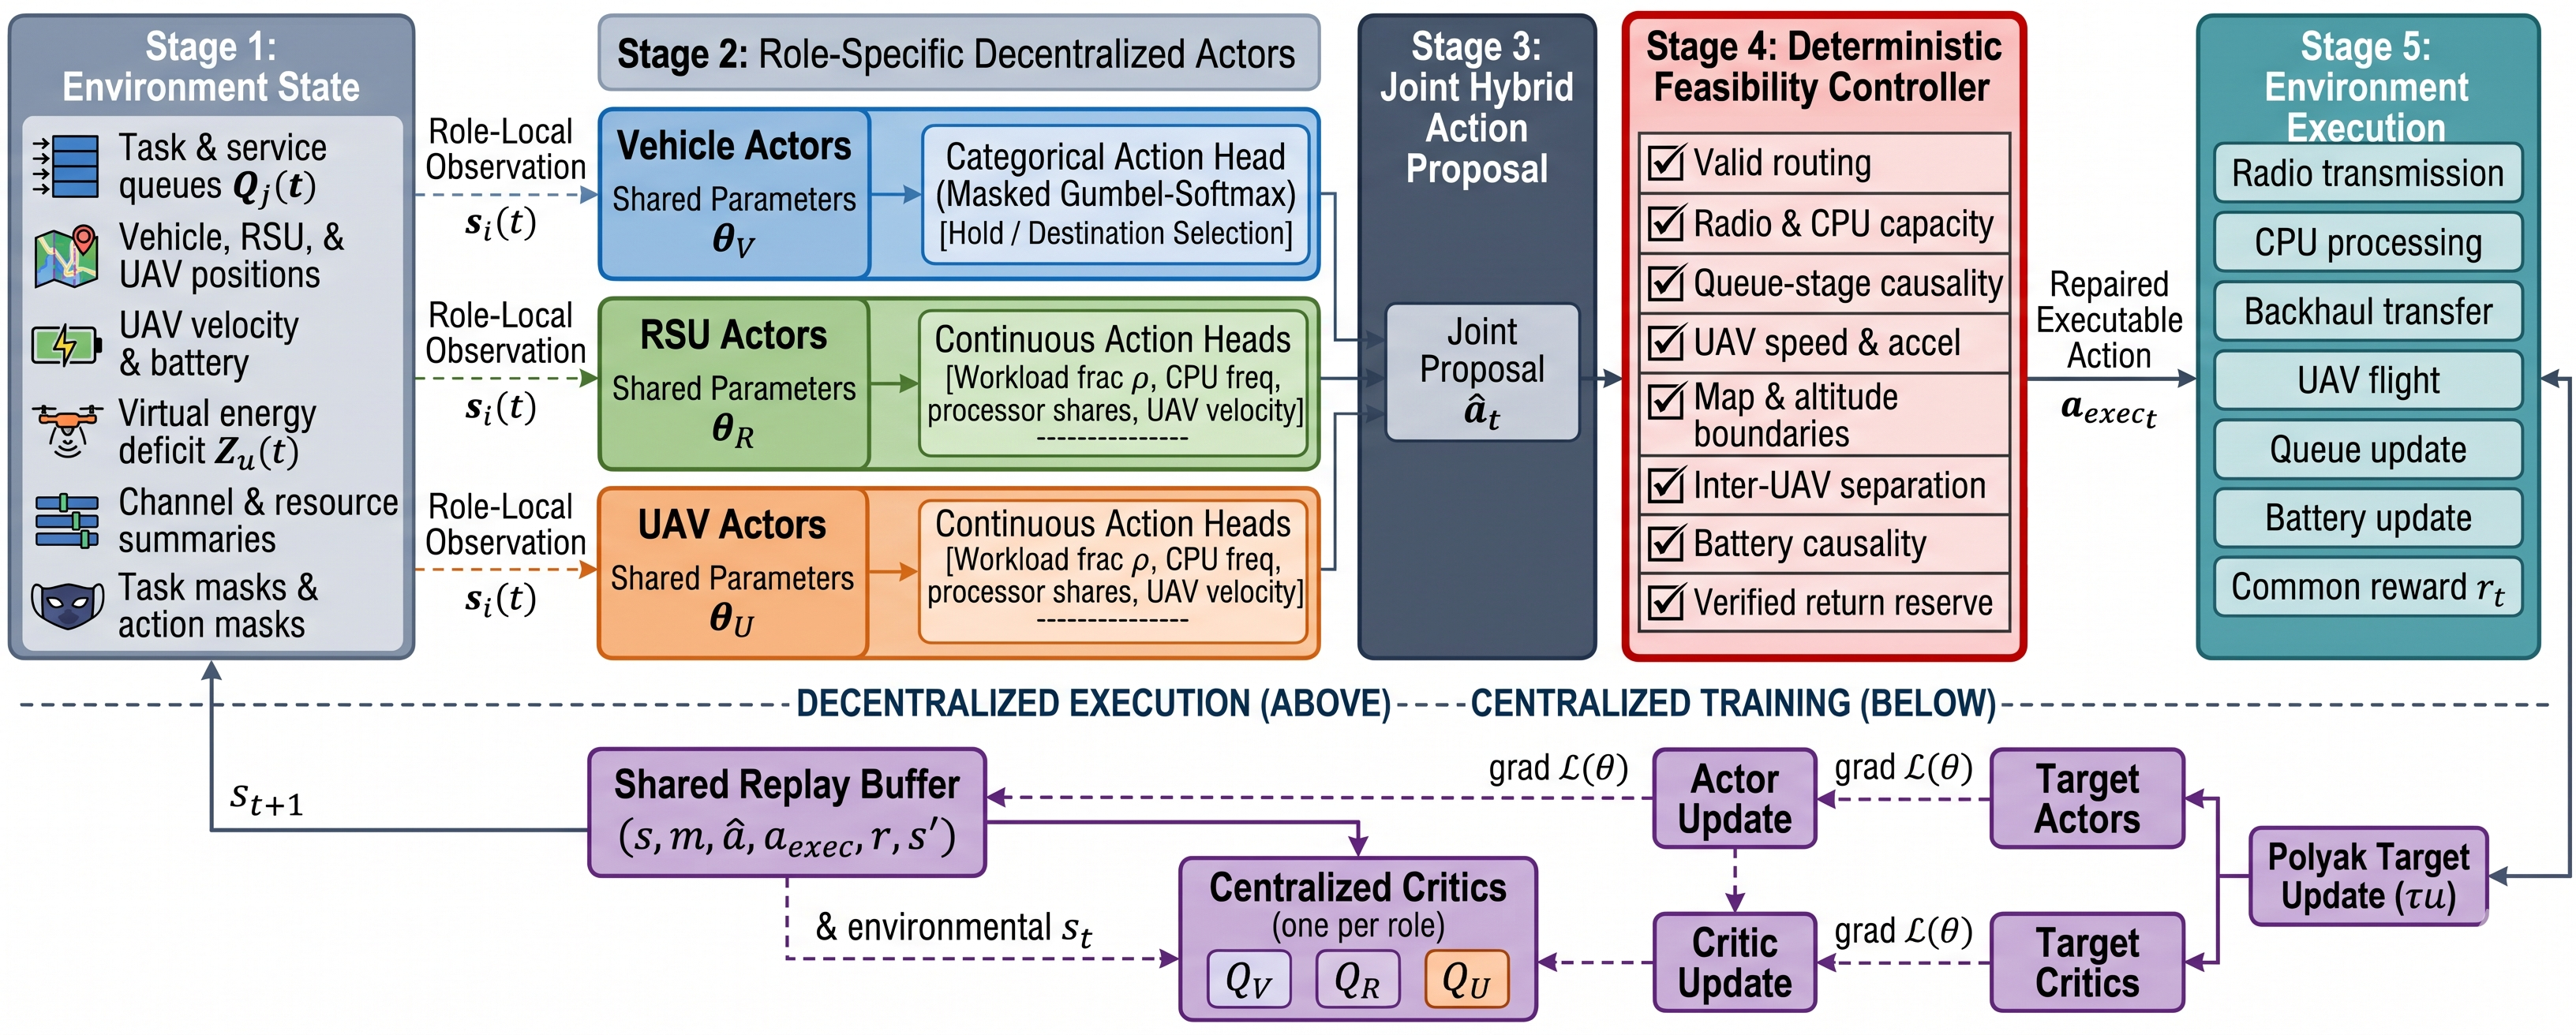
\includegraphics[width=0.98\textwidth]{Complete QA-DR-MADDPG architecture.png}
\caption{Complete \method\ architecture. Vehicle, RSU, and UAV actors use
role-local observations at execution time, whereas centralized critics and
the shared replay buffer are active only during training. The feasibility
controller separates neural proposals from physically executed actions.}
\label{fig:controller_architecture}
\end{figure*}

\subsubsection{Role-Shared Actors and Centralized Critics}
For visible task feature $x_{hi}$ and mask $m_{hi}\in\{0,1\}$, the actor uses
a task encoder and masked pooling,
\begin{align}
e_{hi}&=\phi_g(x_{hi}),\qquad
\bar e_h=\frac{\sum_i m_{hi}e_{hi}}
{\max\{1,\sum_i m_{hi}\}},\nonumber\\
z_h&=\operatorname{LN}\!\left(
\phi_g^{\rm trunk}([o_h;\bar e_h])\right).
\label{eq:actor_encoder}
\end{align}
Actors share parameters within a role but not across roles. One centralized
critic per role evaluates
\begin{equation}
Q_{\psi_g}(s_t,\vect a_t)=q_{\psi_g}([s_t;\operatorname{vec}(\vect a_t)]).
\label{eq:centralized_critic}
\end{equation}

\subsubsection{Categorical and Continuous Action Heads}
For categorical destination logit $l_{hd}$ and feasibility mask $c_{hd}$,
invalid choices receive $-\infty$. During training, the straight-through
Gumbel-softmax output is
\begin{align}
\tilde l_{hd}&=\begin{cases}l_{hd},&c_{hd}=1,\\-\infty,&c_{hd}=0,\end{cases}
\nonumber\\
y_{hd}&=\frac{\exp((\tilde l_{hd}+g_{hd})/\tau_G)}
{\sum_{d'}\exp((\tilde l_{hd'}+g_{hd'})/\tau_G)},\nonumber\\
\hat x_h^{\rm cat}&=\operatorname{sg}
\left(\operatorname{onehot}(\arg\max_d y_{hd})-y_h\right)+y_h,
\label{eq:gumbel_action}
\end{align}
with $g_{hd}=-\log[-\log u_{hd}]$ and $u_{hd}\sim\mathcal U(0,1)$. Evaluation
removes Gumbel noise and uses masked argmax. Continuous heads satisfy
\begin{align}
\rho_i&=\sigma(z_i^\rho),
&f_u&=f_u^{\max}\sigma(z_u^f),\nonumber\\
\hat{\vect u}_u&=\mathcal S_u\tanh(z_u^{\rm mot}),
&w_{hi}&=\frac{m_{hi}e^{z_{hi}^w}}{\sum_jm_{hj}e^{z_{hj}^w}}.
\label{eq:continuous_heads}
\end{align}
Thus partition and frequency remain bounded, motion respects configured
component limits before physical repair, and positive task shares sum to one.

\subsubsection{Feasibility Controller}
Let $\mathcal C(s_t,\hat a_t)$ contain the proposal, scaled motions, and
verified contingencies. The executable action is selected as
\begin{equation}
a_t^{\rm exec}=\mathcal H(s_t,\hat a_t)
\in\arg\min_{a\in\mathcal C(s_t,\hat a_t)\cap\mathcal F(s_t)}
D(a,\hat a_t),
\label{eq:feasibility_projection}
\end{equation}
where $D$ combines categorical disagreement and normalized continuous
distance. The feasible set enforces routing masks, radio/CPU capacity, stage
causality, speed, acceleration, map and altitude limits, continuous-path
separation, battery causality, and return reserve. If normal service is not
admissible, the UAV disables new service and follows a verified return or
landing contingency. Proposal/execution differences and repair frequencies
are retained for evaluation.

\begin{figure*}[!t]
\centering
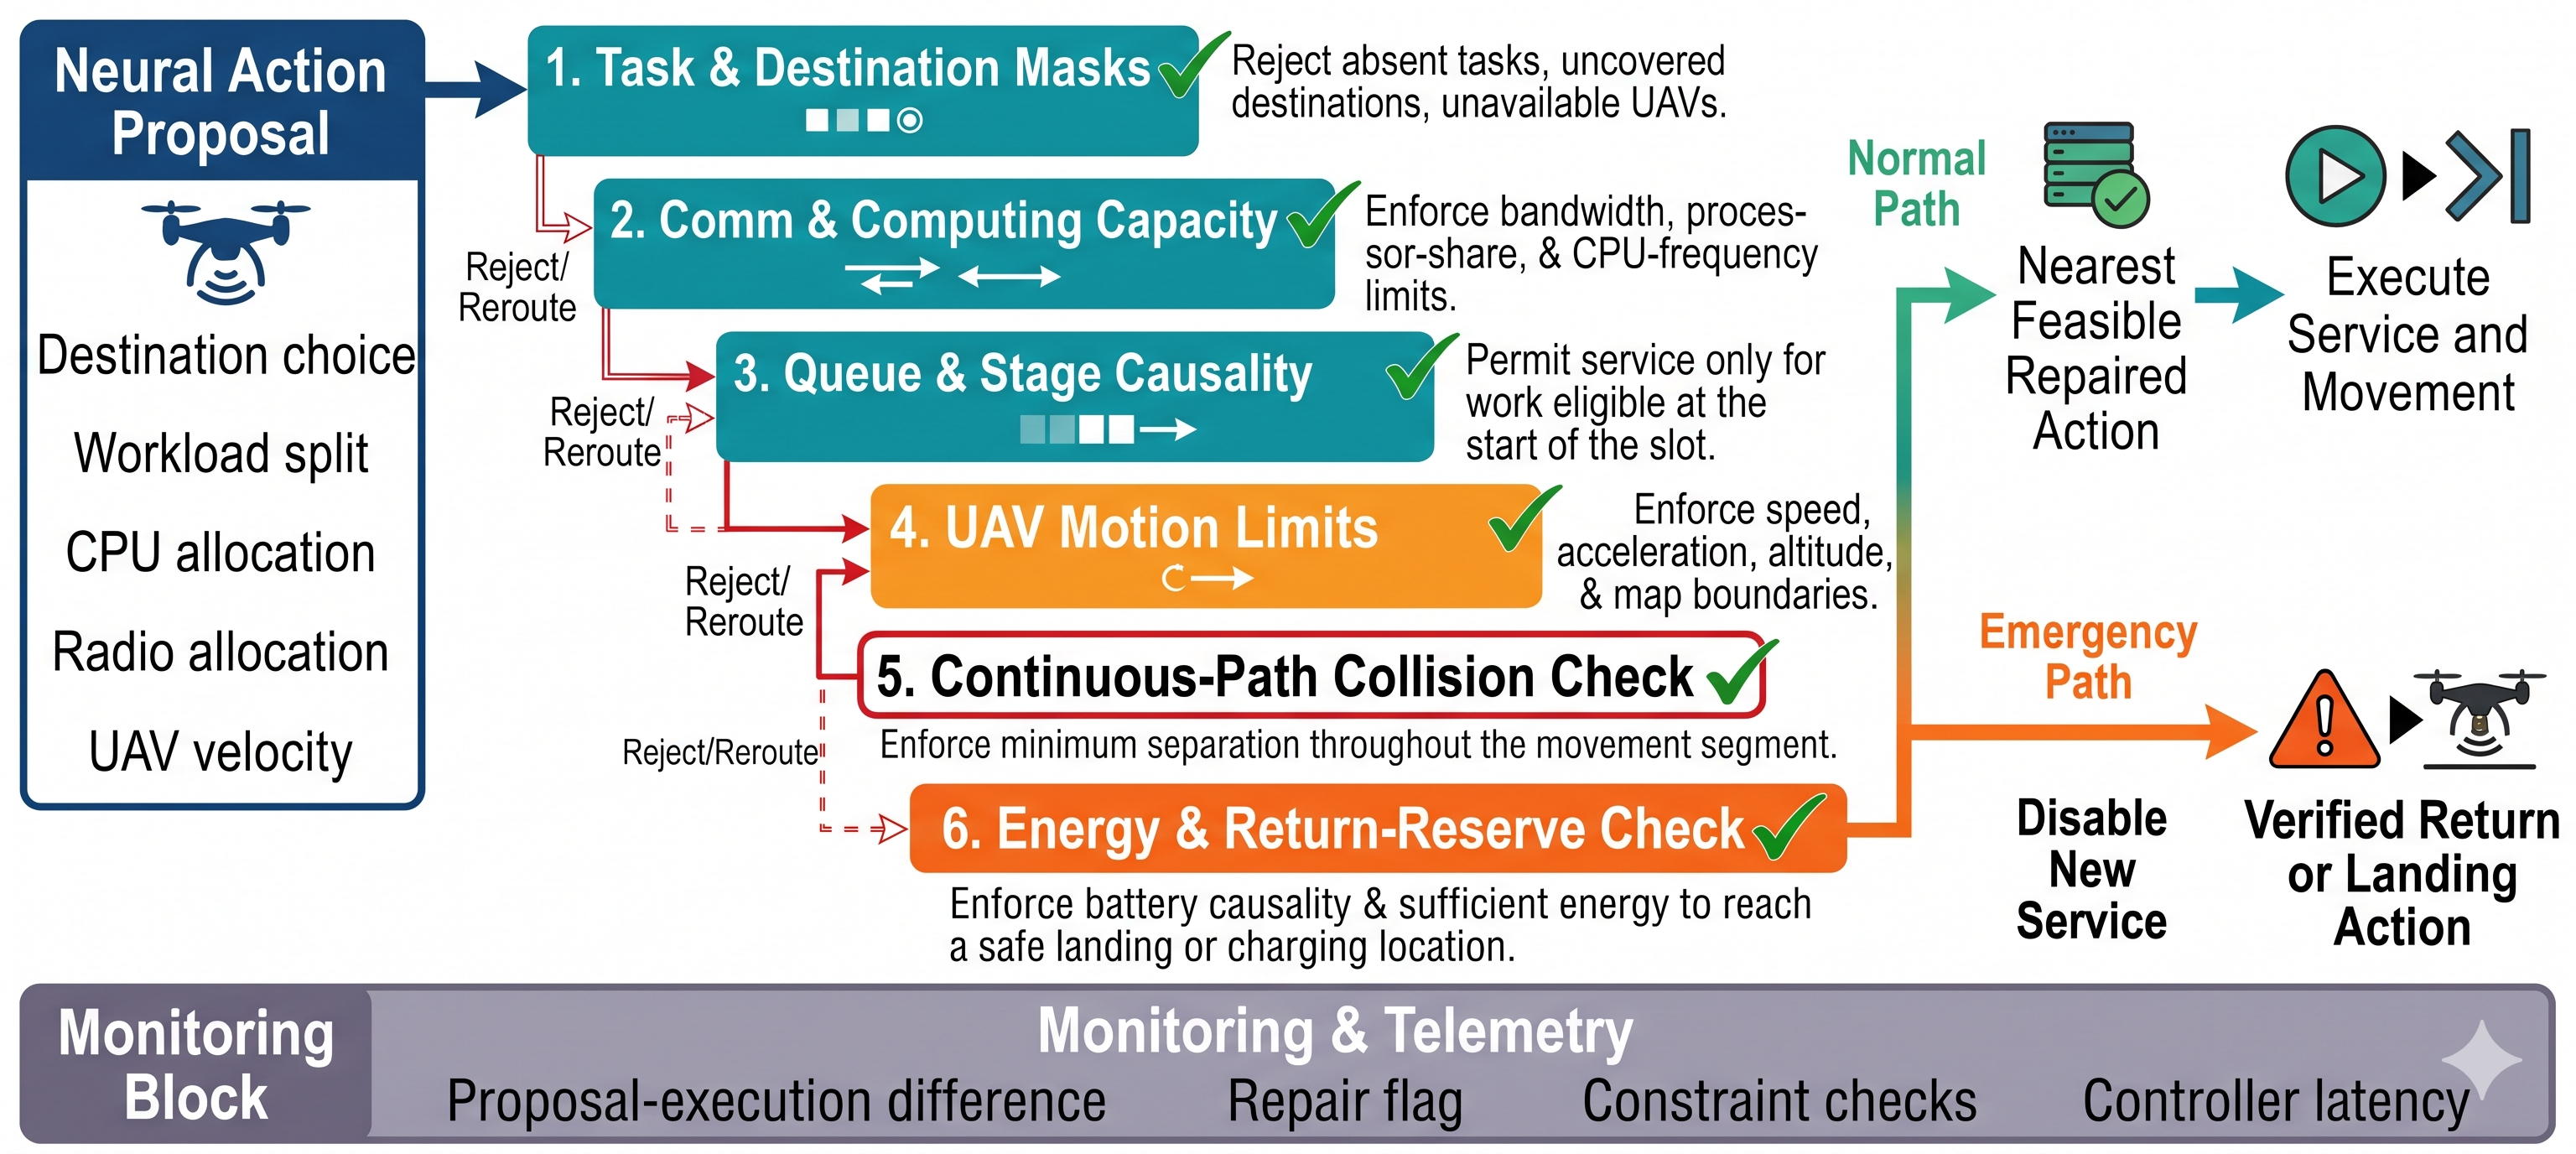
\includegraphics[width=0.95\textwidth]{Feasibility controller and safe-action workflow.png}
\caption{Deterministic feasibility-controller workflow. A neural hybrid
proposal is checked against routing, resource, queue-causality, motion,
continuous-path separation, battery, and return-reserve constraints. The
controller executes the nearest admissible repair or invokes a verified
return or landing contingency.}
\label{fig:feasibility_workflow}
\end{figure*}

\subsubsection{Critic, Actor, and Target Updates}
Replay stores current/next states, role observations, masks, proposed and
executed joint actions, reward, and done flag $d_b$. For minibatch size $B$,
the target and critic loss are
\begin{align}
y_{g,b}&=r_b+\gamma(1-d_b)Q_{\psi_g^-}
(s'_b,\mathcal H_{\rm tens}(\vect a'_b)),\label{eq:critic_target_new}\\
\mathcal L_g(\psi_g)&=\frac1B\sum_{b=1}^{B}
\left(Q_{\psi_g}(s_b,a_b^{\rm exec})-y_{g,b}\right)^2.
\label{eq:critic_loss_new}
\end{align}
For the actor update, role $g$ uses its current proposal while the other roles
retain detached executed replay actions. Denoting this mixed action by
$\tilde a_b^{(g)}$, the maximized objective is
\begin{equation}
J_g=\frac1B\sum_bQ_{\psi_g}(s_b,\tilde a_b^{(g)})
-\lambda_{\rm rep}\frac1B\sum_b
\|\hat a_{g,b}-\operatorname{sg}(a_{g,b}^{\rm exec})\|_2^2.
\label{eq:actor_objective_new}
\end{equation}
The repair term encourages proposals near actions that can actually execute;
the complete physical controller is not differentiated through. After Adam
updates, targets follow
\begin{equation}
\theta_g^-\leftarrow(1-\tau_p)\theta_g^-+\tau_p\theta_g,
\qquad
\psi_g^-\leftarrow(1-\tau_p)\psi_g^-+\tau_p\psi_g.
\label{eq:polyak_new}
\end{equation}
With the reported configuration, training performs one actor--critic update
after each environment transition once replay contains at least 64 samples.

\subsection{Domain-Randomized Training and Deployment}
The completed study defines a scenario domain
\begin{equation}
\omega=(\lambda,H,C^{\rm bh},\xi),
\label{eq:domain_tuple_correct}
\end{equation}
where $\lambda$ specifies load or a traffic change, $H$ specifies nominal,
zero, or interrupted replenishment, $C^{\rm bh}$ is backhaul capacity, and
$\xi$ is the recorded task/harvest random seed. The training manifest contains
$10\times7=70$ scenario specifications. Each epoch samples seven distinct
specifications uniformly without replacement from that manifest. This gives
equal expected exposure across the declared stress classes but does not force
one example of every class in every epoch.

The robust training objective is
\begin{equation}
\max_\Theta\;\E_{\omega\sim p_{\rm train}}
\E_{\tau\sim\pi_\Theta,\omega}
\left[\sum_{t=0}^{T-1}\gamma^t r_t\right].
\label{eq:dr_objective_new}
\end{equation}
All episodes update the same parameters $\Theta$; there are no task-specific
copies or Reptile interpolation. Validation uses 35 disjoint specifications
(five seeds by seven stresses), and checkpoint selection requires improved
mean validation reward with zero modeled physical violations. Early stopping
uses a patience of ten validations.

\begin{figure*}[!t]
\centering
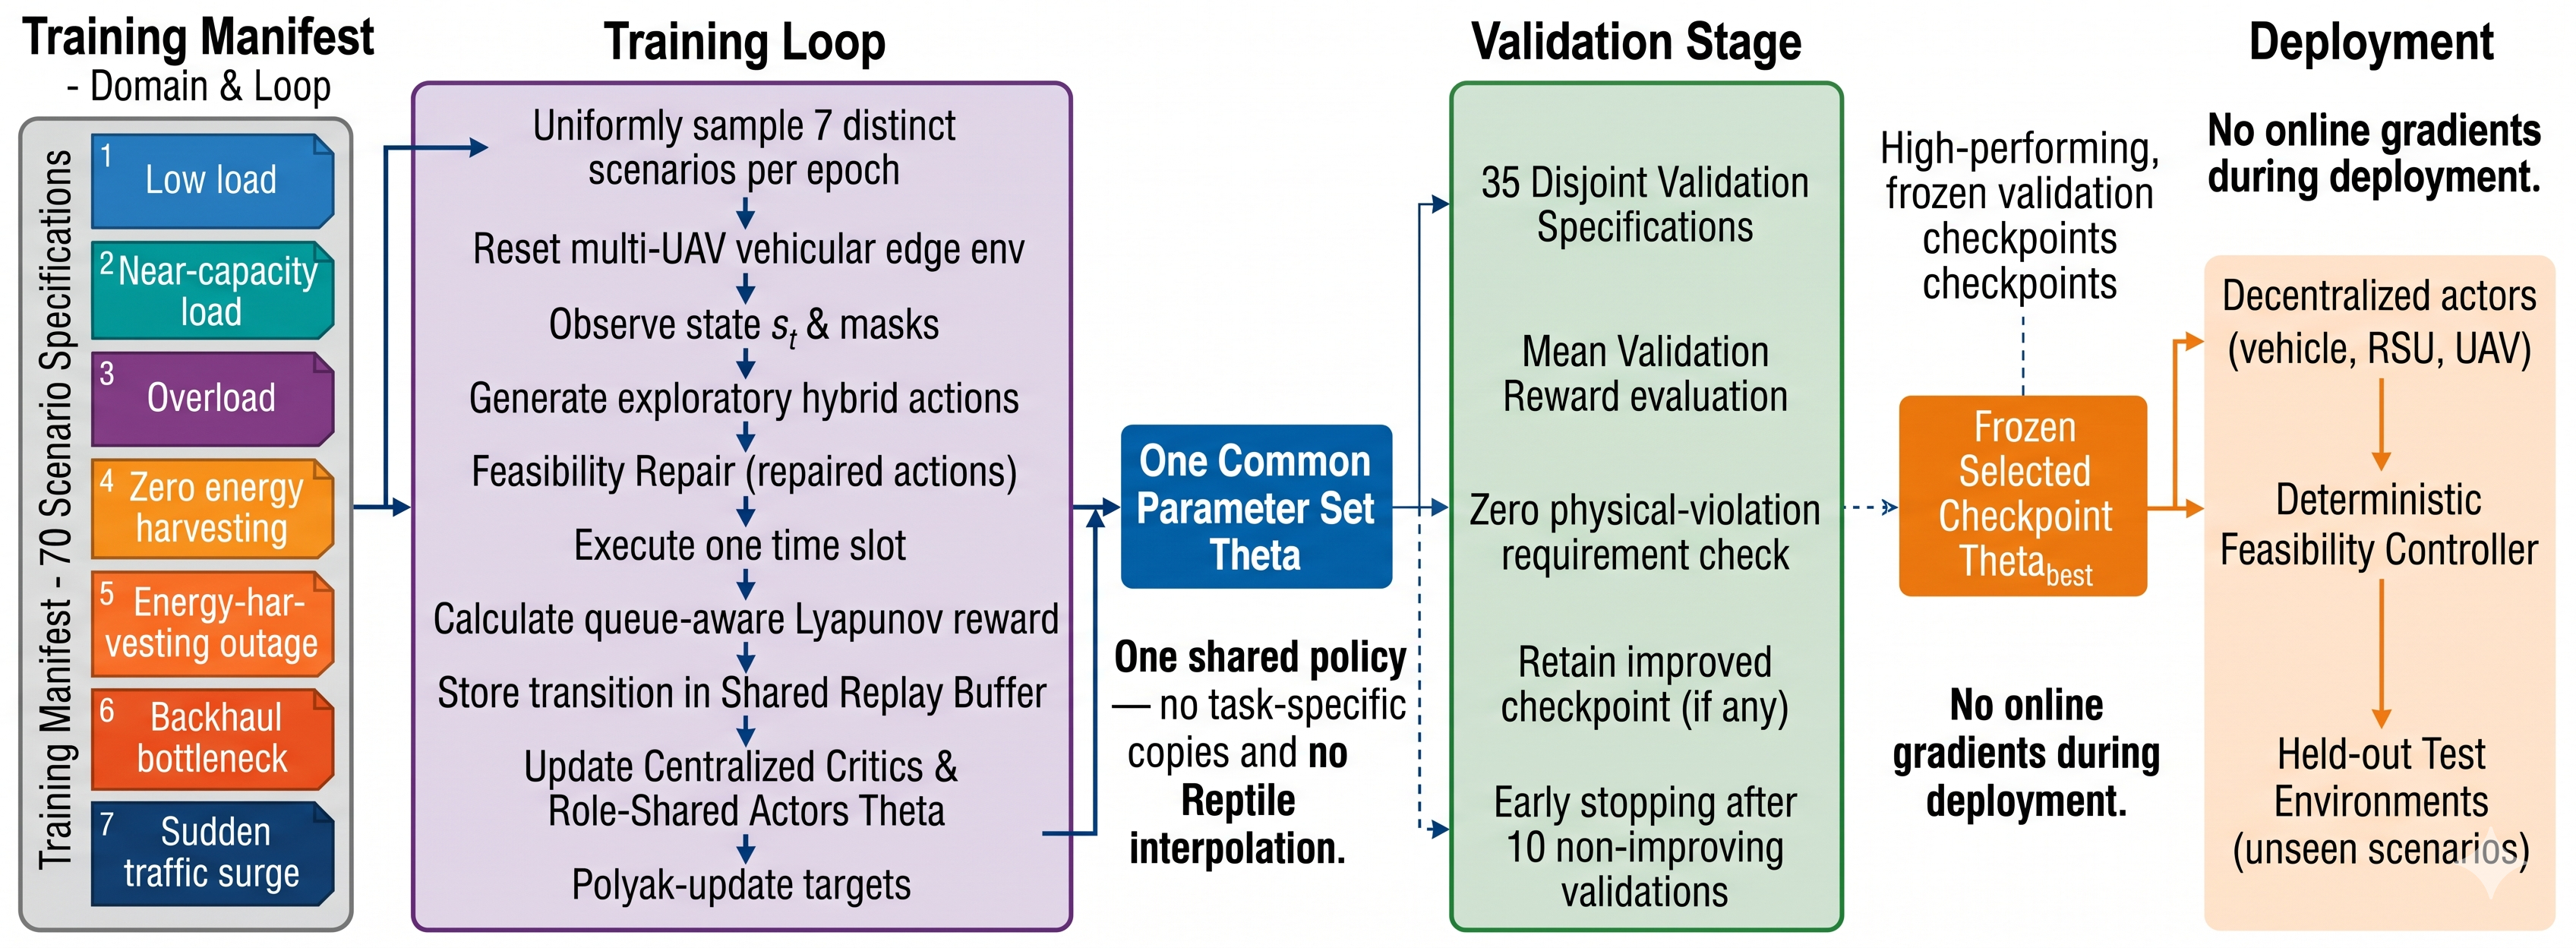
\includegraphics[width=0.98\textwidth]{Domain-randomized training and deployment workflow.png}
\caption{Domain-randomized training, validation, and deployment workflow.
Seven stress classes update one common parameter set; disjoint validation
selects an improved zero-violation checkpoint. Deployment freezes the chosen
actors and disables centralized critics, replay sampling, and gradient
updates.}
\label{fig:dr_workflow}
\end{figure*}

\begin{algorithm}[!t]
\caption{Queue-aware domain-randomized Hybrid MADDPG}
\label{alg:dr_maddpg_new}
\KwIn{Training manifest $\Omega_{\rm tr}$, replay capacity $N$, batch size $B$,
target rate $\tau_p$}
\KwOut{Validation-selected parameters $\Theta^*$}
Initialize online/target actors, critics, and replay $\mathcal D$\;
\For{each epoch $e$}{
 sample seven distinct scenarios $\omega\subset\Omega_{\rm tr}$\;
 \For{each sampled scenario and slot $t$}{
  encode $s_t$, local observations, task masks, and action masks\;
  generate exploratory hybrid proposal $\hat a_t$\;
  execute $a_t^{\rm exec}=\mathcal H(s_t,\hat a_t)$\;
  observe $r_t,s_{t+1}$ and append the complete transition to $\mathcal D$\;
  \If{$|\mathcal D|\ge B$}{
   update all role critics using Eq.~\eqref{eq:critic_loss_new}\;
   update all role actors using Eq.~\eqref{eq:actor_objective_new}\;
   apply Eq.~\eqref{eq:polyak_new}\;
  }
 }
 evaluate the fixed policy on all validation specifications\;
 retain only an improved, zero-violation checkpoint; stop after ten
 non-improving validations\;
}
\end{algorithm}

At deployment, each slot requires a forward pass through the role-local
actors followed by the deterministic feasibility controller. The selected
parameters remain fixed: centralized critics, replay sampling, and gradient
updates are disabled. Evaluation therefore measures how the trained policy
generalizes across the test scenarios without online adaptation.

\subsection{Computational and Storage Complexity}
Let $n_g$, $d_g$, and $a_g$ denote the number of agents, observation width,
and action width of role $g$; $M_{\rm task}$ is maximum visible tasks;
$d_{\rm task}$ is task-feature width; $h_a$ and $h_c$ are actor and critic
hidden widths; $d_s$ is global-state width; and
$d_A=\sum_gn_ga_g$. A joint actor pass has order
\begin{align}
C_\mu=\mathcal O\!\Bigg(\sum_gn_g\big[&
M_{\rm task}(d_{\rm task}h_a+h_a^2)\nonumber\\
&+(d_g+h_a)h_a+h_a^2+h_aa_g\big]\Bigg),
\label{eq:actor_complexity_new}
\end{align}
and one centralized critic per role gives
\begin{equation}
C_Q=\mathcal O\!\left(|\mathcal G|
\left[(d_s+d_A)h_c+h_c^2+h_c\right]\right).
\label{eq:critic_complexity_new}
\end{equation}
One minibatch update is $\mathcal O(B(C_\mu+C_Q))$. If feasibility repair
tests $K_{\rm rep}$ joint candidates at cost $C_{\rm feas}$, its worst-case
slot contribution is $\mathcal O(K_{\rm rep}C_{\rm feas})$. Replay storage is
$\mathcal O(Nd_{\rm tr})$ and network, target-network, gradient, and Adam
state storage is $\mathcal O(P_\Theta)$. Decentralized deployment evaluates no
critic and costs $\mathcal O(C_\mu+K_{\rm rep}C_{\rm feas})$ per slot.
